% Meerkat-TRIZ arXiv paper — single-file LaTeX (article class, standard packages only)
% Compile: pdflatex main && pdflatex main
% Status: author block updated (Ning Yang, Tensoris — cross-family evaluation support); v5b gate results and equal-length control integrated.
\documentclass[11pt]{article}
\usepackage[margin=1in]{geometry}
\usepackage{booktabs}
\usepackage{amsmath}
\usepackage{graphicx}
\usepackage{amssymb}
\usepackage{tikz}
\usetikzlibrary{arrows.meta,positioning}
\usepackage{xcolor}
\usepackage{multirow}
\usepackage{array}
\usepackage[colorlinks=true,linkcolor=blue,citecolor=blue,urlcolor=blue]{hyperref}

\newcommand{\model}{Meerkat-TRIZ}
\newcommand{\tbd}[1]{\textcolor{red}{\textbf{[TBD: #1]}}}

\title{\model: A Fine-Tuned Language Model for TRIZ-Based Inventive
Problem Solving with Dual-Track Evaluation and Cross-Family
Judge Verification}

\author{%
  Jia Luo$^{1,*}$\quad Siyuan Huang$^{2,*}$\quad Ning Yang$^{3}$\\[2pt]
  $^{1}$Meerkat AI\quad $^{2}$Insentek\quad $^{3}$CBCTech\\[2pt]
  \texttt{arthur.lok@innoenterprise.com}\\
  \texttt{siyuan.huang@insentek.com}\\
  \texttt{christina.yang@cbctech.com}\\[2pt]
  \small Model: \url{https://huggingface.co/Meerkat-AI/Meerkat-TRIZ-v1}\\
  \small Code \& benchmark: \url{https://github.com/coidea-sys/meerkat-triz}
}

\date{July 2026}

\begin{document}
\maketitle

\begin{abstract}
TRIZ (Theory of Inventive Problem Solving) is the most widely used
systematic innovation methodology in engineering practice, yet existing
work combining TRIZ with large language models (LLMs) has relied
exclusively on prompting, retrieval, or multi-agent orchestration of
general-purpose models. We present \model, to our knowledge the first
publicly released TRIZ-domain \emph{fine-tuned} LLM: a QLoRA adapter
(0.24\% of parameters) trained on a Qwen3.6-35B-A3B MoE base with an
11k-example curriculum covering six TRIZ task families plus safety
refusals. Because domain claims are only as strong as their measurement,
the paper's second contribution is an evaluation methodology designed to
survive adversarial scrutiny: (i)~\textbf{TRIZ-Bench}, a 300-item
six-task benchmark whose questions and keyword sets are public;
(ii)~a \emph{dual-track} protocol pairing an objective keyword track
with an anti-verbosity LLM-judge track; (iii)~paired-bootstrap
significance testing with fixed seeds throughout; (iv)~a
\emph{cross-family judge panel} with family recusal and a circuit
breaker that freezes shipping when an in-family judge contradicts the
external consensus; and (v)~an eight-gate decision procedure
(G0--G8) that has repeatedly caught regressions that single-metric
leaderboards would have missed. Applying this apparatus, we show that
\model~v1 improves over its 35B base by $+0.39$ ($\pm$0.10, 95\%~CI)
on the in-family judge but only $+0.09$ to $+0.10$ under two external
judges and $-0.05$ under a third---a $\sim$4$\times$ inflation pattern
that would have gone undetected with a single judge. An
\emph{equal-length control} then isolates the residual confound: when
the base is instructed to match the fine-tune's answer length, the
in-family gain vanishes ($-0.07$, n.s.) while the base's own in-family
score rises by $+0.46$ from brevity alone---yet under two of three
\emph{external} judges the same length-matched base falls
\emph{below} the fine-tune by $+0.19$ to $+0.27$ (significant).
Length was masking a genuine content-quality gain: the fine-tune is
better at a level length budget, and at natural lengths delivers that
content at $0.4\times$ the answer length with keyword coverage the
base cannot retain when compressed. On the objective
keyword track, the fine-tune matches its base ($\pm$0.0001) and both
outscore GPT-5.4, Claude~Sonnet~4.6, Claude~Opus~4.8 and
Gemini~3.5~Flash on TRIZ keyword coverage; on the judge track the best
frontier models still lead, with Claude~Opus~4.8 scoring significantly
\emph{below} the 35B base. A 120-item general-ability probe shows no
significant capability sacrifice from domain fine-tuning
($-1.25$pp vs.\ predecessor, floor $-5$pp). We release the model, the
evaluation harness, the public benchmark, and all judge caches to make
every number in this paper recomputable.
\end{abstract}

\section{Introduction}
\label{sec:intro}

TRIZ (\emph{Teoriya Resheniya Izobretatelskikh Zadach}, Theory of
Inventive Problem Solving), developed by Altshuller from the analysis of
hundreds of thousands of patents, codifies invention as the resolution
of \emph{contradictions}: improving one engineering parameter while
avoiding the degradation of another, using 40 inventive principles, a
contradiction matrix, separation principles, and the ARIZ algorithm.
Despite its industrial adoption, TRIZ remains expertise-bound: mapping a
messy real-world problem onto the correct standard contradiction, and
then committing to the right principles with defensible justification,
is precisely the step practitioners find hardest.

Large language models are a natural vehicle for lowering this barrier,
and several groups have explored the combination
\cite{autotriz,trizgpt,trizagents,gusarov2026}. All of these works,
however, treat the LLM as a general-purpose reasoner steered by prompts,
retrieval, or agent pipelines. None trains the model on the domain, and
none evaluates with the statistical machinery that the LLM-as-judge
literature has shown to be necessary \cite{mtbench,panickssery2024}.
Two questions therefore remain open: (1)~does domain fine-tuning
actually move TRIZ task quality beyond what a strong base model or a
frontier model already achieves? and (2)~how should such a claim be
measured when the most convenient instrument---an LLM judge from the
same model family that generated the training data---is itself suspect?

This paper answers both. Our contributions are:

\begin{enumerate}
  \item \textbf{The first public TRIZ fine-tuned LLM.} \model~v1 is a
  QLoRA adapter on Qwen3.6-35B-A3B (MoE, 256 routed experts; adapters on
  12 shared projections, 0.24\% of parameters), trained on an
  11k-example, seven-subset curriculum. Model, training configuration,
  and data-construction pipeline are public.
  \item \textbf{A measurement-first evaluation methodology.} Dual-track
  scoring (objective keyword track $+$ anti-verbosity judge track),
  paired-bootstrap inference with fixed seeds, a 120-item
  general-ability probe, and an eight-gate shipping decision procedure
  (G0--G8) whose gates are machine-checkable and whose backtests
  reproduce our past ship/no-ship decisions exactly.
  \item \textbf{Cross-family judge verification.} A panel of external
  judges from three vendors, with family recusal (a judge never scores
  its own family's generations) and a circuit breaker (G8) that blocks
  shipping when in-family and external verdicts contradict. We quantify
  the resulting correction: the in-family judge's headline effect
  ($+0.39$) deflates to $+0.09$/$+0.10$/$-0.05$ under external judges,
  while external judges agree with each other at Spearman
  0.63--0.75 but only 0.27--0.31 with the in-family judge. An
  equal-length generation control completes the correction---and then
  reverses it upward: once the base is instructed to match the
  fine-tune's answer length, the in-family effect vanishes ($-0.07$,
  n.s.), exposing the headline as predominantly a length artifact,
  while two of three external judges score the fine-tune significantly
  \emph{above} the length-matched base ($+0.19$/$+0.27$), isolating a
  genuine content-quality gain that length had masked.
  \item \textbf{A frontier baseline.} TRIZ-Bench results for GPT-5.4,
  Claude Sonnet~4.6, Claude Opus~4.8, and Gemini~3.5~Flash under the
  identical protocol, with per-judge disclosure of every number.
  \item \textbf{A documented failure-driven iteration lineage.} Five
  model generations (v2$\to$v5b), each changed by a single variable and
  each decided by the gates, including three rejected generations and the
  attribution analyses that rejected them---evidence that the
  methodology, not luck, produces the improvement
  (Figure~\ref{fig:lineage}).
\end{enumerate}

\begin{figure}[t]
\centering
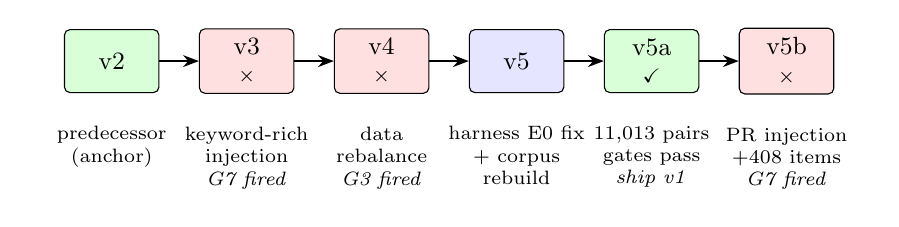
\begin{tikzpicture}[
  font=\small,
  node distance=3mm and 5mm,
  gen/.style={draw, rounded corners=2pt, minimum width=12mm,
              minimum height=8mm, align=center},
  ok/.style={gen, fill=green!15},
  rej/.style={gen, fill=red!12},
  fix/.style={gen, fill=blue!10},
  pend/.style={gen, fill=gray!15, dashed},
  note/.style={align=center, font=\scriptsize, text width=19mm},
  arr/.style={-{Stealth[length=2mm]}, thick}
]
\node[ok] (v2) {v2};
\node[rej, right=of v2] (v3) {v3\\[-1pt]\scriptsize $\times$};
\node[rej, right=of v3] (v4) {v4\\[-1pt]\scriptsize $\times$};
\node[fix, right=of v4] (v5) {v5};
\node[ok, right=of v5] (v5a) {v5a\\[-1pt]\scriptsize $\checkmark$};
\node[rej, right=of v5a] (v5b) {v5b\\[-1pt]\scriptsize $\times$};
\draw[arr] (v2) -- (v3);
\draw[arr] (v3) -- (v4);
\draw[arr] (v4) -- (v5);
\draw[arr] (v5) -- (v5a);
\draw[arr] (v5a) -- (v5b);
\node[note, below=of v2] {predecessor\\ (anchor)};
\node[note, below=of v3] {keyword-rich\\ injection\\ \emph{G7 fired}};
\node[note, below=of v4] {data\\ rebalance\\ \emph{G3 fired}};
\node[note, below=of v5] {harness E0 fix\\ $+$ corpus\\ rebuild};
\node[note, below=of v5a] {11{,}013 pairs\\ gates pass\\ \emph{ship v1}};
\node[note, below=of v5b] {PR injection\\ $+$408 items\\ \emph{G7 fired}};
\end{tikzpicture}
\caption{Single-variable lineage v2$\to$v5b. Each generation changes
exactly one factor (annotated below); red generations were rejected by
the decision gates, blue repaired the measurement harness, and green
shipped as \model~v1.}
\label{fig:lineage}
\end{figure}

Section~\ref{sec:related} positions against prior TRIZ$\times$LLM work
and the LLM-as-judge literature. Section~\ref{sec:model} describes data
and training. Section~\ref{sec:eval} defines the evaluation apparatus.
Section~\ref{sec:results} reports results, including the frontier
leaderboard. Section~\ref{sec:analysis} analyzes failure modes and judge
bias. Section~\ref{sec:limits} is an unusually detailed limitations
section; Section~\ref{sec:concl} concludes.

\section{Related Work}
\label{sec:related}

\paragraph{TRIZ meets LLMs: prompting, not training.}
AutoTRIZ \cite{autotriz} automates TRIZ ideation by prompt-structured
LLM calls and evaluates on textbook cases; TRIZ-GPT \cite{trizgpt}
compares prompt strategies for GPT-3.5/4 inside a TRIZ workflow;
TRIZ Agents \cite{trizagents} decomposes the methodology across a
multi-agent pipeline; Gusarov \cite{gusarov2026} frames TRIZ as a
reasoning scaffold for materials science with local models. Common
traits: the model weights are never touched; evaluation is by case
study or heuristic LLM scoring without significance testing; and no
public benchmark exists. Our work is complementary in spirit---we keep
TRIZ's structured problem formulation as the task definition---but
orthogonal in mechanism: domain adaptation through supervised
fine-tuning, with measurement treated as a first-class deliverable.

\paragraph{Domain fine-tuning.}
Parameter-efficient fine-tuning \cite{lora,qlora} has made single-GPU
domain adaptation routine. What remains rare is discipline in what is
claimed from it. Our training recipe is deliberately plain (QLoRA, fixed
hyperparameters, two-epoch cosine horizon); the novelty is not the
optimizer but the decision procedure around it: every generation changes
one variable and must pass eight machine-checkable gates.

\paragraph{LLM-as-judge and its biases.}
Zheng et al.\ \cite{mtbench} established LLM judging at scale and
documented position and verbosity biases; Panickssery et al.\
\cite{panickssery2024} showed evaluators favor their own generations;
length-controlled variants of automatic arenas \cite{alpacaeval} exist
precisely because judges reward length. Our design imports these
lessons: an anti-verbosity clause in the rubric, position-swap
validation in harness development, fixed-temperature scoring, and---most
importantly---treating any single judge, especially one from the data
generator's family, as a hypothesis to be falsified by external judges
rather than as ground truth.

\paragraph{Benchmarks and contamination.}
Holistic multi-metric evaluation \cite{helm}, live refreshed benchmarks
\cite{livebench}, and public reproducible harnesses motivate our
release shape: public questions and keyword sets, withheld reference
answers, documented decontamination (character 3-gram Jaccard,
threshold 0.5, with a 0.4--0.5 human-review band), versioned snapshots,
and full judge-cache disclosure so that every table cell can be
recomputed independently.

\section{Model and Training}
\label{sec:model}

\subsection{Base model and adapter}
\model~v1 attaches QLoRA adapters \cite{lora,qlora} ($r{=}64$,
$\alpha{=}128$, dropout 0, RSLoRA off) to twelve shared projection
modules (\texttt{q,k,v,o\_proj}, \texttt{in\_proj\_qkv,z,b,a},
\texttt{out\_proj}, \texttt{gate,up,down\_proj}) of Qwen3.6-35B-A3B
\cite{qwen3}, a
Mixture-of-Experts base with 256 routed experts. Only 0.24\% of
parameters are trainable; the routed experts themselves are untouched.
Training is supervised fine-tuning \cite{instructgpt} in pure BF16 on a single
unified-memory accelerator, batch 1
$\times$ grad-accum 8, lr $2{\times}10^{-4}$ with a cosine schedule
whose horizon is two epochs (four-epoch cap as safety), max sequence
2048, completion-only loss, seed 42. Hyperparameters were fixed by a
small sweep at an earlier generation and then \emph{frozen}: every
subsequent generation changes data only, preserving single-variable
comparability across the lineage (Table~\ref{tab:lineage}).

\subsection{Training data}
The v5-line corpus derives from a cleaned collection of Chinese TRIZ
textbooks, courseware, and proceedings, expanded by model-generated
long-form answers under hard quality gates (length bands, tail-template
blacklists, dedup) and decontaminated against the evaluation gold set by
character 3-gram Jaccard ($\geq$0.5 drop; 0.4--0.5 human review).
The final v5b training set contains 11{,}421 prompt--completion pairs in
seven subsets: concept explanation (2{,}996), innovation assessment
(3{,}037), case generation (2{,}857), ARIZ guidance (1{,}442),
contradiction analysis (313), principle recommendation (521), and
safety refusal (255).

The principle-recommendation subset deserves note because it is the
paper's running case study (Section~\ref{sec:analysis}). Attribution on
the previous generation found the subset to be the smallest (196 items),
72\% of it ``concise-mode'' items capped at 300 characters, and---most
damning---42\% mislabeled (ARIZ resource questions, standard-solution
questions, and patent-analysis questions carrying a
principle-recommendation tag). The v5b generation audits out the 83
mislabeled items and injects 408 newly generated examples whose answers
must commit to specific numbered principles with justification, pass a
hedging filter (``may involve/one may consider'' phrasing rejected),
cover all 40 inventive principles without omission, and pass gold-set
decontamination.

\begin{table}[t]
\centering
\small
\caption{Model lineage. Each row changes exactly one variable relative
to its predecessor; ship/reject verdicts are produced by the G0--G8
gates (Section~\ref{sec:gates}).}
\label{tab:lineage}
\begin{tabular}{@{}llll@{}}
\toprule
Generation & Change & Gate verdict & Note \\
\midrule
v2 & v5-line corpus rebuild & ship & baseline predecessor \\
v3 & keyword-rich data push & \textbf{reject} & judge track regressed \\
v4 & data rebalance & \textbf{reject} & concept-explanation $-8$ kw \\
v5 & new gold + corpus & superseded & training-protocol defect \\
v5a & protocol fix (E0) & \textbf{ship} (as v1) & released model \\
v5b & PR audit $+$ injection & \textbf{reject} & G7 fired $\times$2; no external confirmation \\
\bottomrule
\end{tabular}
\end{table}

\section{Evaluation Methodology}
\label{sec:eval}

\subsection{TRIZ-Bench}
The benchmark contains 300 Chinese items in six task families
(concept explanation, contradiction analysis, principle recommendation,
ARIZ guidance, case generation, innovation assessment; 30--60 items per
family), each with a question, a reference answer, and an expected
keyword set. Questions and keyword sets are public (CC-BY-NC); reference
answers are withheld to slow benchmark decay. Generation protocol for
all models is identical: one TRIZ-expert system message, max 2048 new
tokens, deterministic decoding where the API allows.

\subsection{Dual-track scoring}
\paragraph{Keyword track (objective).} Per-item hit rate of expected
keywords under a curated alias map (substring plus confirmed synonyms),
fully deterministic and recomputable by anyone from the public files.

\paragraph{Judge track (semantic), Arm A.} An LLM judge scores each
answer 0--4 on five dimensions (accuracy, completeness, TRIZ
correctness, structure, overall) against the reference answer, with an
explicit anti-verbosity clause (``length is not evidence of quality''),
full untruncated input, temperature 0, five items per request, batch
parse failures degrading to single-item retries, and a fixed judge
system prompt. An Arm B variant judging only same-length-bucket pairs
exists for length-confound control, but with only 17/300 qualifying
pairs it is underpowered; we report Arm A and treat the length confound
as an open measurement debt (Section~\ref{sec:limits}).

\subsection{Inference}
All comparisons are paired at item level: paired bootstrap on per-item
differences (10{,}000 resamples, seed 42), McNemar's exact test for
pass-rate asymmetries, Wilson intervals for rates, and Spearman's
$\rho$ for judge--judge agreement. No claim in this paper is made
without a confidence interval; ``significant'' always means a 95\% CI
excluding zero.

\subsection{Cross-family judge panel and recusal}
Every arm is scored by the in-family judge (Moonshot) and by external
judges from three vendors (Claude, GPT, Gemini families). Two rules
make the panel adversarial: \emph{family recusal}---a judge never
scores generations of its own family---and \emph{full per-judge
disclosure}---no averaging across judges, because averaging hides
exactly the disagreement we want to inspect.

\subsection{Decision gates G0--G8}
\label{sec:gates}
Shipping is decided by eight machine-checkable gates applied to the
paired statistics: G0 over-refusal $\leq$2\%; G1 vs-base judge CI lower
bound $>-0.15$; G2 vs-predecessor CI lower bound $>-0.05$ with at least
one track significantly positive; G3 keyword-regression attribution
(distinguishing true regressions from scoring artifacts); G4 small-cell
($n{<}30$) subsets are descriptive only; G5 ARIZ rubric precedence; G6
general-ability probe degradation $>-5$pp; G7 dual-track contradiction
circuit breaker (tracks significantly opposing); G8 cross-family
contradiction circuit breaker (in-family significantly positive while
all or a majority of external judges are significantly negative $\Rightarrow$
fail). Any FAIL keeps the predecessor; any SKIP freezes the release
pending data. Backtests of the gate suite reproduce all historical
ship/reject decisions, including the two rejections in
Table~\ref{tab:lineage}.

\subsection{General-ability probe}
A 120-item six-category general Chinese probe (no TRIZ content) is run
on base, predecessor, and candidate under a neutral system prompt, to
detect capability sacrifice from domain tuning.


\section{Results}
\label{sec:results}

\subsection{Fine-tune vs.\ base: the judge you choose changes the answer}
Table~\ref{tab:main} is the paper's central table. Under the in-family
judge, \model~v1 (v5a) improves over base by $+0.393$
[$+0.297$, $+0.490$] on the 0--4 scale---a headline any single-judge
paper would print. Under external judges the same paired differences
are $+0.094$ [$+0.020$, $+0.167$] (Claude), $+0.104$
[$+0.020$, $+0.184$] (GPT), and $-0.048$ [$-0.144$, $+0.045$]
(Gemini): two significantly positive but $\sim$4$\times$ smaller, one
indistinguishable from zero. The direction survives verification; the
magnitude does not (Figure~\ref{fig:inflation}). Even this deflated
pattern has a residual length confound---base answers are much longer
than the fine-tune's---and Section~\ref{sec:eqlen} shows that under an
equal-length control the in-family difference disappears entirely,
while two of three \emph{external} judges on the same matched arm find
the fine-tune significantly \emph{better}; we restate the fine-tune's
benefit accordingly. Meanwhile the objective keyword track is an exact
tie ($0.6384$ vs $0.6383$, diff $-0.0001$ n.s.), so we report the
honest composite: the fine-tune adds judged quality without adding
keyword coverage, and the size of the quality gain depends on who
judges---and, under the in-family judge, on how long the answers are.

\begin{table}[t]
\centering
\small
\caption{\model~v1 (v5a) vs.\ base on TRIZ-Bench (300 items). Judge
cells: paired diff [95\% CI] from 10{,}000 paired-bootstraps, seed 42.
$^*$CI excludes zero.}
\label{tab:main}
\begin{tabular}{@{}lcc@{}}
\toprule
Track / judge & diff (v5a $-$ base) & sig. \\
\midrule
Keyword (objective) & $-0.0001$ & n.s. \\
Moonshot (in-family) & $+0.393$ [$+0.297$, $+0.490$] & $^*$ \\
Claude Sonnet 4.6 & $+0.094$ [$+0.020$, $+0.167$] & $^*$ \\
GPT-5.4 & $+0.104$ [$+0.020$, $+0.184$] & $^*$ \\
Gemini 3.5 Flash & $-0.048$ [$-0.144$, $+0.045$] & n.s. \\
\bottomrule
\end{tabular}
\end{table}

\begin{figure}[t]
\centering
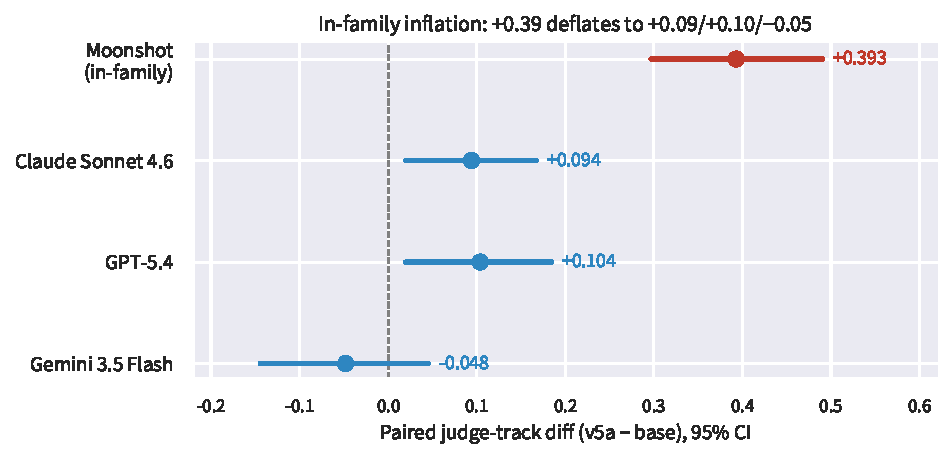
\includegraphics[width=0.9\linewidth]{figures/fig_judge_inflation.pdf}
\caption{The in-family inflation pattern at a glance. Paired judge-track
differences (v5a $-$ base) with 95\% CIs under each judge. The in-family
judge's headline $+0.393$ deflates to $+0.094$/$+0.104$/ $-0.048$ under
three external judges---the direction survives, the magnitude does
not.}
\label{fig:inflation}
\end{figure}

Judge--judge agreement explains why the correction matters
(Table~\ref{tab:spearman}, Figure~\ref{fig:agreement}). External judges cohere with each other
($\rho$ 0.63--0.75) at roughly the level MT-Bench reports for
GPT-4-vs-human agreement, but barely cohere with the in-family judge
($\rho$ 0.27--0.31). The in-family judge is not merely more generous;
it is measuring something related but different---consistent with
self-preference findings \cite{panickssery2024}, and the reason G8
exists.

\begin{table}[t]
\centering
\small
\caption{Judge--judge Spearman $\rho$ on the base arm (300 items).}
\label{tab:spearman}
\begin{tabular}{@{}lc@{}}
\toprule
Pair & $\rho$ \\
\midrule
Claude $\sim$ GPT & 0.738 \\
GPT $\sim$ Gemini & 0.692 \\
Claude $\sim$ Gemini & 0.628 \\
\midrule
Moonshot $\sim$ any external & 0.27--0.31 \\
\bottomrule
\end{tabular}
\end{table}

\begin{figure}[t]
\centering
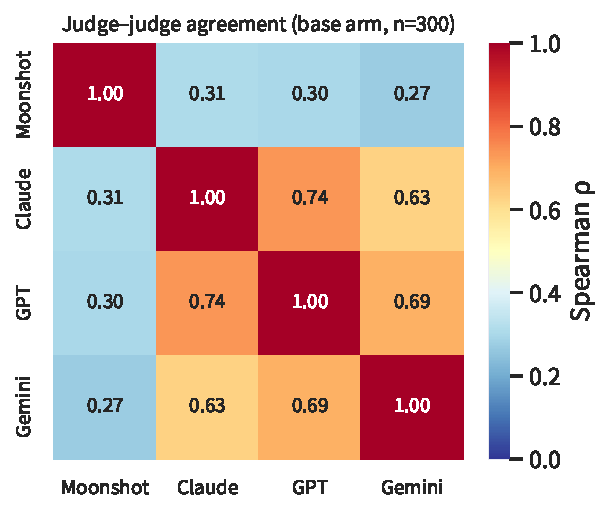
\includegraphics[width=0.62\linewidth]{figures/fig_judge_agreement.pdf}
\caption{Judge--judge Spearman $\rho$ on the base arm ($n{=}300$).
External judges form a coherent block (0.63--0.75); the in-family judge
barely correlates with any of them (0.27--0.31)---it is measuring
something related but different.}
\label{fig:agreement}
\end{figure}

\subsection{Frontier models on TRIZ-Bench}
\label{sec:frontier}
We ran GPT-5.4, Claude Sonnet 4.6, Claude Opus 4.8, and Gemini 3.5
Flash as \emph{contestants} under the identical protocol (5{,}983 valid
scores; seven item-level scores lost to API safety refusals and treated
as missing, never zero). Table~\ref{tab:leaderboard} condenses the full
per-judge matrix.

\begin{table}[t]
\centering
\small
\caption{TRIZ-Bench contestant table. kw: keyword hit rate. Judge cells:
overall mean (paired diff vs.\ base [95\% CI]); ``---'' marks family
recusal.}
\label{tab:leaderboard}
\begin{tabular}{@{}lccccc@{}}
\toprule
Contestant & kw & Claude & Gemini & GPT & Moonshot \\
\midrule
base & 0.638 & 2.555 & 2.871 & 2.301 & 3.030 \\
\model~v1 & 0.638 &
  2.649 ($+$0.09$^*$) & 2.823 ($-$0.05) & 2.405 ($+$0.10$^*$) & 3.423 ($+$0.39$^*$) \\
GPT-5.4 & 0.628 &
  2.692 ($+$0.14$^*$) & 3.094 ($+$0.23$^*$) & --- & 3.213 ($+$0.18$^*$) \\
Sonnet 4.6 & 0.576 &
  --- & 2.846 ($-$0.04) & 2.299 ($-$0.02) & 3.080 ($+$0.05) \\
Opus 4.8 & 0.576 &
  --- & 2.776 ($-$0.10) & 2.204 ($-$0.10) & 2.572 ($-$0.46$^*$) \\
Gemini 3.5F & 0.599 &
  2.863 ($+$0.31$^*$) & --- & 2.587 ($+$0.29$^*$) & 3.268 ($+$0.23$^*$) \\
\bottomrule
\end{tabular}
\end{table}

Three findings stand out. First, on the \emph{objective} track the 35B
base and its fine-tune beat every frontier model we tested---domain
keyword coverage is where specialization shows up with certainty.
Second, on the judge track the strongest frontier models (Gemini,
GPT-5.4) still lead the fine-tune; their answers are longer and more
elaborately structured, and judges---even with an anti-verbosity
rubric---reward some of that. We read the residual gap as partly real
(elaboration quality) and partly the known length confound
(Section~\ref{sec:limits}); v5b's targeted injection attacked the real
part and was nonetheless rejected by the gates
(Section~\ref{sec:v5b}). Third, Claude Opus 4.8 scores \emph{below} the 35B base
on every judge that is allowed to score it, and significantly so on the
in-family judge ($-0.458$ [$-0.575$, $-0.344$])---a reminder that
frontier general models do not automatically dominate narrow
methodological domains, and a result we could not have credibly
published without the recusal-and-disclosure protocol.

\subsection{General ability is not sacrificed}
On the 120-item general probe: base 84.03\%, predecessor (v2) 86.81\%,
\model~v1 85.56\%. The candidate-vs-predecessor difference of $-1.25$pp
is far above the G6 floor ($-5$pp), and the candidate sits
\emph{above} base. Domain fine-tuning at 0.24\% of parameters did not
buy domain skill with general regression.

\subsection{The v5b case study: a correctly rejected repair}
\label{sec:v5b}
Section~\ref{sec:analysis} attributes the previous generation's
principle-recommendation weakness to three data defects. v5b tested the
repair with a single-variable change: 408 injected commit-style items
(length band 800--1600 characters, all 40 inventive principles covered,
gold-decontaminated) plus removal of the 83 mislabeled items, for
11{,}421 training pairs; every other subset was byte-identical to v5a
and every hyperparameter was frozen.

The repair worked \emph{behaviorally} and failed \emph{measurably}.
Qualitatively, v5b no longer hedges: sampled principle-recommendation
answers now commit to numbered principles with application logic
(``Principle one: segmentation\ldots''), exactly the deficit the
attribution identified. Quantitatively, the gates rejected the
generation on two independent significant track-reversals
(Table~\ref{tab:v5b}). Against base, the in-family judge-track gain
grew to $+0.430$ while the objective track went significantly
\emph{negative} ($-0.028$); against v2 on the targeted subset the same
flip appeared in extreme form (judge $+0.800$ vs.\ keyword $-0.135$).
G7 fired. The external panel made the rejection unambiguous: all three
external judges scored v5b statistically indistinguishable from base
($+0.067$/$-0.003$/$+0.015$, all n.s.), so unlike v5a---whose small
gain two of three external judges confirmed---v5b's larger in-family
headline has \emph{zero} external confirmation.

\begin{table}[t]
\centering
\small
\caption{v5b dual-track outcome (paired diffs, 95\% CI). The two
significant reversals that fired G7 are marked $\dagger$.}
\label{tab:v5b}
\begin{tabular}{@{}lcc@{}}
\toprule
Comparison & judge track & keyword track \\
\midrule
v5b $-$ base, overall$\dagger$ & $+0.430$ [$+0.323$, $+0.537$] &
  $-0.028$ [$-0.048$, $-0.009$] \\
v5b $-$ base, principle rec.\ & $-0.033$ [$-0.217$, $+0.167$] &
  $-0.104$ [$-0.159$, $-0.049$] \\
v5b $-$ v2, principle rec.$\dagger$ & $+0.800$ [$+0.617$, $+1.000$] &
  $-0.135$ [$-0.193$, $-0.082$] \\
\midrule
External judges (v5b $-$ base) & \multicolumn{2}{c}{claude $+0.067$ n.s.;
  gpt $-0.003$ n.s.; gemini $+0.015$ n.s.} \\
\bottomrule
\end{tabular}
\end{table}

Attribution of the keyword regression found it to be primarily a
measurement artifact rather than degraded principle selection. Of 59
lost keyword instances on the 60-item subset, only 22\% are
principle-name mismatches (v5b recommending, e.g., segmentation where
the reference chose prior action); 78\% are generic framing tokens
(\emph{TRIZ}, \emph{inventive principle}, \emph{technical
contradiction}) that base's longer answers sprinkle and the terse
commit-style format omits. v5b in fact hits expected keywords at
\emph{higher} density than base (1.88 vs.\ 1.03 per 1{,}000
characters); its absolute hit count falls because its answers are
0.39$\times$ as long (median 1{,}055 vs.\ 2{,}792 characters), and a
counterfactual holding base's density fixed attributes the entire net
drop to this length surface. The objective track thus measures a
length-sensitive vocabulary contract rather than what the injection
changed; meanwhile all judges, external included, scored the two arms
equal, so no judged-quality gain offsets the contract loss. The decision gates' verdict---G7 fail, G3
freeze pending formal attribution---is that this trade is not worth
making: v5b is rejected, and \model~v1 (v5a) remains the shipped model.
We report v5b in detail precisely because a single-metric pipeline
would have shipped it: its in-family headline ($+0.430$) is the largest
in the lineage. Section~\ref{sec:eqlen} later shows that both of v5b's
significant tracks against base decompose into length-surface effects.

\subsection{The equal-length control}
\label{sec:eqlen}
Section~5.1 leaves one confound standing: base answers are much longer
than v5a's (median 3{,}242 vs.\ 1{,}344 characters), and the in-family
rubric explicitly penalizes verbosity. If the rubric works, part of
v5a's $+0.393$ could be a length artifact rather than a quality gain.
An earlier attempt to isolate the effect by score-bucket pairing was
underpowered (17/300 same-bucket pairs), so we ran a direct control:
base regenerated all 300 items with a per-item length target equal to
v5a's answer length on that item (``keep the answer to about $N$
characters $\pm 10\%$''), every other protocol element byte-identical;
judging and inference are unchanged.

Length compliance was partial. The instruction asked for a median of
1{,}344 characters; base produced a median of 1{,}750 (1.29$\times$
overshoot; 20/300 items inside the $\pm 10\%$ band), compressing the
base-to-v5a length ratio from 2.4$\times$ to 1.3$\times$. We report
the control as-is rather than iterating toward perfect compliance.

\begin{table}[t]
\centering
\small
\caption{Equal-length control, in-family judge (0--4), paired diffs
with 95\% CIs (10{,}000 paired bootstraps, seed 42). Row~1 recomputes
Table~\ref{tab:main} on the control's paired sample and reproduces it
exactly; rows~4--5 apply the same control to the rejected v5b
generation at zero additional generation cost.}
\label{tab:eqlen}
\begin{tabular}{@{}lc@{}}
\toprule
Comparison & diff [95\% CI] \\
\midrule
v5a $-$ base (unconstrained) & $+0.393$ [$+0.297$, $+0.490$] \\
v5a $-$ base (length-matched) & $-0.070$ [$-0.140$, $+0.000$] \\
base (matched) $-$ base (unconstrained) & $+0.463$ [$+0.367$, $+0.557$] \\
\midrule
v5b $-$ base (unconstrained) & $+0.430$ [$+0.323$, $+0.537$] \\
v5b $-$ base (length-matched) & $-0.033$ [$-0.110$, $+0.043$] \\
\bottomrule
\end{tabular}
\end{table}

Table~\ref{tab:eqlen} separates artifact from gain for the in-family
judge, and two conclusions stand. First, \textbf{v5a's in-family
advantage does not survive length control}: with base constrained
toward v5a's length the paired difference is $-0.070$ and statistically
null---the $+0.393$ headline is predominantly a length artifact. Mean
scores make the mechanism visible: base 3.030 unconstrained, 3.493
length-matched, v5a 3.423. Second, \textbf{the anti-verbosity rubric
is real}: base's only change was a length instruction, and its judged
score rose by $+0.463$---the judge penalizes verbosity itself, not
capability.

\begin{table}[t]
\centering
\small
\caption{The equal-length control under \emph{external} judges (v5a
$-$ base, paired diffs [95\% CI], $n{=}299$). Matched-arm CIs are
additionally widened by judge rerun-noise synthesis
(Section~\ref{sec:limits}, rule D6): Claude [$+0.105$, $+0.270$], GPT
[$+0.161$, $+0.380$]---both remain significant.}
\label{tab:eqlen_ext}
\begin{tabular}{@{}lcc@{}}
\toprule
Judge & unconstrained & length-matched \\
\midrule
Claude Sonnet 4.6 & $+0.094$ [$+0.020$, $+0.167$] & $\mathbf{+0.187}$ [$+0.110$, $+0.264$] \\
GPT-5.4 & $+0.104$ [$+0.020$, $+0.184$] & $\mathbf{+0.271}$ [$+0.177$, $+0.368$] \\
Gemini 3.5 Flash & $-0.048$ [$-0.144$, $+0.045$] & $+0.025$ [$-0.074$, $+0.120$] \\
\bottomrule
\end{tabular}
\end{table}

Third, \textbf{the external judges reverse the picture---upward}
(Table~\ref{tab:eqlen_ext}). Scoring the same matched-length arm, two
of three external judges rate v5a significantly \emph{above} base. The
mechanism mirrors the in-family one with the sign flipped: external
judges \emph{lower} base's score when it is forced to write short
(GPT $2.301 \to 2.134$; Claude $2.555 \to 2.462$)---they reward
elaboration, so base's unconstrained sprawl was itself buying judged
quality. At a level length budget the fine-tune's content is genuinely
better; base closes most of the gap only by spending $2.4\times$ the
tokens, and even then not all of it (the unconstrained residuals
$+0.09$/$+0.10$ of Section~5.1). The four readings now compose a
single consistent picture: in-family $+0.39$ (anti-verbosity
over-credits) $\to$ in-family matched $-0.07$ (rubric real but
conservative) $\to$ external unconstrained $+0.09$/$+0.10$ (length and
content offset) $\to$ external matched $+0.19$/$+0.27$ (content
quality, isolated).

The keyword track sharpens rather than
contradicts this: unconstrained, v5a and base are tied ($-0.0001$
n.s.), but length-matched base \emph{loses} keyword coverage relative
to its unconstrained self ($-0.023$ [$-0.040$, $-0.005$]) while v5a
does not---so at matched length v5a significantly \emph{out-covers}
base on keywords ($+0.023$ [$+0.005$, $+0.041$]). Brevity costs the
base keyword surface that the fine-tune retains at $0.4\times$ the
length. The same control applied to the rejected v5b generation
(Table~\ref{tab:eqlen}, rows~4--5) dissolves \emph{both} of its
significant tracks: the judge gain ($+0.430 \to -0.033$ n.s.) and the
keyword loss ($-0.028 \to -0.006$ n.s.) are alike length-surface
effects---v5b's behavioral change is real, but every measured effect
against base was a length phenomenon (its regression against v2 on the
targeted subset is not length-controlled here and stands).

The claim this paper makes is therefore stronger than parity: at
matched length the fine-tune outperforms its base under two of three
external judges, and at natural lengths it delivers that content at
$0.4\times$ the answer length with keyword coverage the base cannot
retain when compressed. We now require an equal-length control as a
mandatory companion to any judge-track significance claim (harness
rule D5), external panel included.

\section{Analysis}
\label{sec:analysis}

\subsection{What was actually wrong with principle recommendation}
The previous generation's weakest subset illustrates why measurement
must precede data work. Four judges agreed the fine-tune did not beat
base on principle recommendation ($+0.05$, $+0.05$, $-0.08$ n.s.;
$-0.31$ significant negative). Attribution found three independent
defects: (i)~\emph{quantity}---196 training items, the smallest domain
subset; (ii)~\emph{style}---72\% of them concise-mode items capped at
300 characters, teaching terseness on a task whose gold answers argue;
(iii)~\emph{labels}---42\% mislabeled, including ARIZ resource
questions and standard-solution questions. Qualitatively, the model had
learned to answer ``recommend two principles'' prompts with a
\emph{methodology lecture} (``step one, restate the contradiction; step
two, consult the matrix\ldots''), hedging instead of committing, while
the base model committed to numbered principles with application logic
and was rewarded for it. The keyword track being significantly
\emph{positive} ($+0.049$) on the same subset proves the model knew the
vocabulary; what it lacked was the behavior, because the behavior
existed in only 54 training examples (Figure~\ref{fig:pr}).

\begin{figure}[t]
\centering
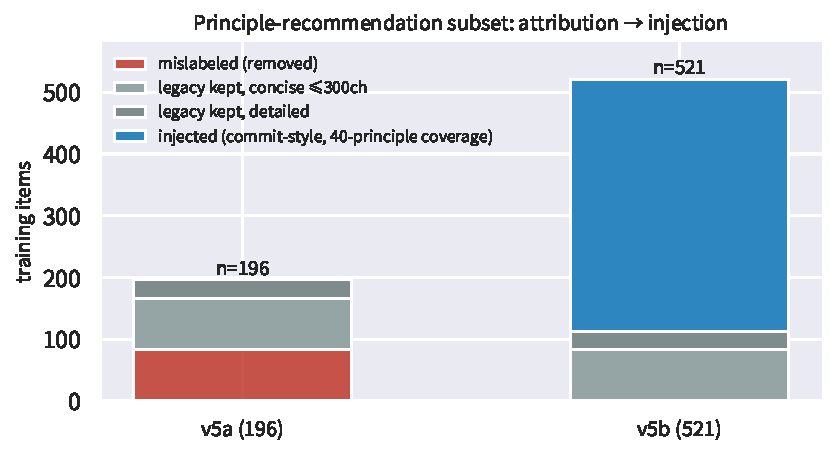
\includegraphics[width=0.72\linewidth]{figures/fig_pr_attribution.pdf}
\caption{Principle-recommendation subset before and after
attribution-driven injection. Left: the v5a subset (196 items) decomposed
by the audit---83 mislabeled items removed, 83 concise-mode and 30
detailed legacy items kept. Right: the v5b subset (521 items) adds 408
injected commit-style items covering all 40 inventive principles. All
other subsets are byte-identical between v5a and v5b.}
\label{fig:pr}
\end{figure}

\subsection{Lessons the gates enforced}
Three rejected generations anchor the methodology's value. v3 pushed
keyword-rich data: the objective track improved and the judge track
significantly regressed---the G7 circuit breaker fired, and attribution
showed keyword stuffing had degraded answer quality. v4 rebalanced data
and quietly dropped eight expected keywords in concept explanation
(true regression, not artifact): G3 fired. v5b repaired a documented
behavioral deficit and produced the lineage's largest in-family
headline ($+0.430$)---and was rejected when the objective track flipped
sign on two comparisons and no external judge confirmed the gain
(Section~\ref{sec:v5b}). All three rejections were of
generations that single-metric evaluation would have shipped. The
counter-discipline also matters: frozen hyperparameters made every
comparison single-variable, and the decision to never ``tune the
learning rate'' when a data fix was available is why the lineage reads
as a sequence of interpretable experiments rather than a soup.

\subsection{Judge bias, mapped}
Our measurements localize four judge biases in this domain:
\emph{family inflation} ($\sim$4$\times$ effect-size deflation when
moving from in-family to external judges);
\emph{leniency offset} (Gemini scores all arms $\sim$0.3--0.6 higher
than GPT while agreeing on rankings, $\rho{=}0.69$);
\emph{elaboration preference} (frontier models' judge-track advantage
co-occurring with 2--3$\times$ answer length despite an anti-verbosity
rubric); and, newly evidenced by v5b, \emph{data-generator--judge
family alignment}: v5b's injected training data was generated by a
model of the same family as the in-family judge, and its in-family
headline \emph{grew} ($+0.430$ vs.\ v5a's $+0.393$) while external
confirmation collapsed to zero ($+0.067$/$-0.003$/$+0.015$ n.s.).
Family bias thus propagates through the data chain, not only the
generation chain: when an intervention's data comes from family $X$, a
family-$X$ judge is doubly compromised, and only the external panel is
insulated. The first two biases are handled by recusal plus disclosure;
the third is now resolved by the equal-length control
(Section~\ref{sec:eqlen}), which shows the in-family rubric's
verbosity penalty is genuine, that the fine-tune's in-family
advantage is predominantly a length artifact---and, symmetrically,
that external judges \emph{lower} the length-matched base (GPT
$2.301 \to 2.134$), a direct measurement of elaboration preference
that isolates the fine-tune's content-quality gain
($+0.19$/$+0.27$); the fourth is handled by treating any same-family
intervention as automatically suspect under G8.

\section{Limitations}
\label{sec:limits}
(i)~The judge-track effect is judge-dependent; the length-matched
external spread ($+0.03$ to $+0.27$) is our best estimate of the true
content-quality effect, but it inherits each judge's rubric
idiosyncrasies. Relatedly, the external judges---served through an API
gateway---are \emph{not} deterministic at temperature~0 (per-item flip
rates 0.18--0.80 over three repeated runs of 50 items; the in-family
judge, called directly, had flip rate 0.000). Published external
differences were computed without judge rerun variance; re-widening
the CIs by rerun-noise synthesis leaves the significant results
significant ($+0.104 \to [+0.006, +0.202]$; $+0.094 \to [+0.015,
+0.173]$; matched-arm $+0.187$/$+0.271$ likewise survive), but
single-run external numbers should be read with this noise budget in
mind (harness rule D6 now gates judge determinism). (ii)~The length confound
on the judge track is bounded but not perfectly removed: the
equal-length control (Section~\ref{sec:eqlen}) overshot its per-item
targets by 29\% (median 1{,}750 vs.\ 1{,}344 characters), and a
stricter-compliance replication is future work. (iii)~The benchmark is
Chinese-only and TRIZ-specific; nothing here tests cross-lingual or
cross-domain transfer. (iv)~Public benchmark questions derive from
copyrighted source texts (model-generated derivatives); we publish
questions and keywords but not reference answers, and a clean-room
v2 benchmark plus an English subset is planned. (v)~Human-expert
validation of judge reliability is scheduled (30-item blind paired
study) but not yet complete at submission time; judge--human agreement
is therefore asserted by proxy (inter-judge agreement), not measured.
(vi)~A single base model and a single adapter configuration are tested;
routed-expert coverage and rank ablations are open engineering
questions. (vii)~v5b, the most recent generation and the only attempted
data-level repair, was rejected by the gates
(Section~\ref{sec:v5b}): how to fix principle recommendation in a way
that satisfies both tracks remains an open problem. Preference
optimization on judge-verified pairs (e.g., DPO \cite{dpo}) is a natural
next step but is deliberately deferred until judge reliability is
human-validated, to avoid distilling a judge's idiosyncrasies into
weights.

\section{Conclusion}
\label{sec:concl}
We set out to answer whether a TRIZ-domain fine-tune is real, and built
the measurement apparatus required to make the answer checkable. The
answer is: real on the objective track, where the fine-tune matches
its base and both beat every frontier model we tested; real as judged
quality \emph{efficiency}---at natural lengths it delivers its content
at $0.4\times$ the base's answer length---and, once length is
controlled, real as a judged-quality \emph{gain}: two of three
external judges score the fine-tune significantly above the
length-matched base ($+0.19$/$+0.27$), even though the in-family
headline itself proved to be a length artifact
(Section~\ref{sec:eqlen}); achieved
without general-capability sacrifice; and
improving through a gated, failure-driven data lineage rather than
through training heroics. We release model, harness, benchmark, and
caches. If the field adopts one habit from this paper, we hope it is
this: never let the family that generated the data be the only judge of
the model---and never print a judge-track gain without a length
control.

\appendix
\section{Generation and judging configurations}
All contestant generations use the system message: ``You are a TRIZ
innovation-methodology expert assistant; answer professionally in
Chinese on TRIZ theory, inventive principles, contradiction analysis and
ARIZ'' (translated), max 2048 tokens. Judges use the Arm-A rubric with
five 0--4 dimensions, batch size 5, temperature 0, full untruncated
input; batch parse failures degrade to single-item retries; API safety
refusals are logged as missing. All bootstrap procedures use
\texttt{random.Random(42)} with 10{,}000 resamples. Judge caches for
every arm$\times$judge cell are published alongside the harness.

\section{Gate definitions (machine-checkable)}
G0: refusal-template hit rate $\leq 2\%$. G1: vs-base Arm-A CI lower
bound $> -0.15$ (Arm B must not contradict). G2: vs-predecessor CI
lower bound $> -0.05$ and (judge or keyword significantly positive).
G3: any subset keyword CI upper bound $<0$ requires attribution;
true-missing $\Rightarrow$ FAIL, artifact $\Rightarrow$ judge-track
arbitration. G4: $n<30$ subsets descriptive only. G5: ARIZ track
divergence resolved for the rubric track. G6: probe diff $> -5$pp.
G7: any dimension with both tracks significant in opposite directions
$\Rightarrow$ FAIL. G8: missing external review $\Rightarrow$ SKIP;
in-family significantly positive with all-external significantly
negative $\Rightarrow$ FAIL; majority-external significantly negative
$\Rightarrow$ FAIL.

\begin{thebibliography}{99}

\bibitem{autotriz}
S.~Jiang and J.~Luo.
\newblock AutoTRIZ: Artificial ideation with TRIZ and large language
  models.
\newblock \emph{arXiv:2403.13002}, 2024.

\bibitem{trizgpt}
\newblock TRIZ-GPT: An LLM-augmented method for problem-solving.
\newblock \emph{arXiv:2408.05897}, 2024.

\bibitem{trizagents}
K.~Szczepanik and J.~Chudziak.
\newblock TRIZ Agents: A multi-agent LLM approach for TRIZ-based
  innovation.
\newblock \emph{arXiv:2506.18783}, 2025.

\bibitem{gusarov2026}
S.~Gusarov.
\newblock Integrating the theory of inventive problem solving with large
  language models: Enhancing reasoning for innovation in materials
  science at the molecular scale.
\newblock \emph{Preprints} 202602.1398, 2026.

\bibitem{mtbench}
L.~Zheng et al.
\newblock Judging LLM-as-a-judge with MT-Bench and Chatbot Arena.
\newblock \emph{NeurIPS} (arXiv:2306.05685), 2023.

\bibitem{panickssery2024}
A.~Panickssery, S.~Bowman, and S.~Feng.
\newblock LLM evaluators recognize and favor their own generations.
\newblock \emph{NeurIPS} (arXiv:2404.13076), 2024.

\bibitem{alpacaeval}
Y.~Dubois et al.
\newblock Length-controlled AlpacaEval: A simple way to debias automatic
  evaluators.
\newblock \emph{arXiv:2404.04475}, 2024.

\bibitem{helm}
P.~Liang et al.
\newblock Holistic evaluation of language models (HELM).
\newblock \emph{arXiv:2211.09110}, 2022.

\bibitem{livebench}
C.~White et al.
\newblock LiveBench: A challenging, contamination-limited LLM benchmark.
\newblock \emph{arXiv:2406.19314}, 2024.

\bibitem{lora}
E.~J. Hu et al.
\newblock LoRA: Low-rank adaptation of large language models.
\newblock \emph{arXiv:2106.09685}, 2021.

\bibitem{qlora}
T.~Dettmers et al.
\newblock QLoRA: Efficient finetuning of quantized LLMs.
\newblock \emph{arXiv:2305.14314}, 2023.

\bibitem{qwen3}
Qwen Team.
\newblock Qwen3 technical report.
\newblock \emph{arXiv:2505.09388}, 2025.

\bibitem{instructgpt}
L.~Ouyang et al.
\newblock Training language models to follow instructions with human
  feedback.
\newblock \emph{arXiv:2203.02155}, 2022.

\bibitem{dpo}
R.~Rafailov et al.
\newblock Direct preference optimization: Your language model is secretly
  a reward model.
\newblock \emph{arXiv:2305.18290}, 2023.

\bibitem{altshuller}
G.~Altshuller.
\newblock \emph{The Innovation Algorithm: TRIZ, Systematic Innovation and
  Technical Creativity}.
\newblock Technical Innovation Center, 1999.

\end{thebibliography}

\end{document}
